%
% ME4140 - Fall 2016
% ROS by Tristan Hill - Tutorials for TnTech Students
% Virtualizing Ubuntu

\documentclass[12pt]{article}
\usepackage{hyperref}
\usepackage[pdftex]{graphicx}
\usepackage{multirow}
\usepackage{setspace}
\usepackage{color}
\usepackage{multicol}

\hypersetup{
    bookmarks=true,         % show bookmarks bar?
    unicode=false,          % non-Latin characters in Acrobat’s bookmarks
    pdftoolbar=true,        % show Acrobat’s toolbar?
    pdfmenubar=true,        % show Acrobat’s menu?
    pdffitwindow=false,     % window fit to page when opened
    pdfstartview={FitH},    % fits the width of the page to the window
    pdftitle={My title},    % title
    pdfauthor={Author},     % author
    pdfsubject={Subject},   % subject of the document
    pdfcreator={Creator},   % creator of the document
    pdfproducer={Producer}, % producer of the document
    pdfkeywords={keyword1, key2, key3}, % list of keywords
    pdfnewwindow=true,      % links in new PDF window
    colorlinks=true,       % false: boxed links; true: colored links
    linkcolor=red,          % color of internal links (change box color with linkbordercolor)
    citecolor=green,        % color of links to bibliography
    filecolor=magenta,      % color of file links
    urlcolor=blue           % color of external links
}

\textwidth=6.5in
\topmargin=-0.5in
\textheight=9.25in
\hoffset=-0.5in
\footskip=0.2in

\pagestyle{myheadings}
\markright{{\large ME 4140 Fall 2019---Virtualizing Ubuntu Linux with Virtual Box}}

\newcommand{\homeWeight}{10}
\newcommand{\quizWeight}{20}
\newcommand{\examWeight}{15}
\newcommand{\finalWeight}{25}

\begin{document}

\thispagestyle{plain}

\begin{center}
   {\bf \Large ROS - Virtualizing Ubuntu Linux with Virtual Box}\vspace{3mm} \\
   {\bf \large ME 4140 - Introduction to Robotics - Fall 2019} \\
\end{center}


\begin{description}
	\vspace{5mm}
 	\item[What is a \href{https://en.wikipedia.org/wiki/Virtual_machine}{Virtual Machine} ?]: \vspace{5mm} \\
      		
\includegraphics[scale=.4]{CaptureA.png}\\
            \begin{itemize}
                
                \item A VM is an Operating System that is {\it virtualized} in your native operating system
                \item this is very useful for experimenting and learning 
                \item not perfect for permanent use
                \item can be resource intensive
                \item \href{https://www.virtualbox.org/}{VirtualBox} is a popular application used for this process
                
            \end{itemize}
	\newpage
		\item[VirtualBox Installation and Setup]: \vspace{10mm} \\


	\begin{enumerate}
\item  Aquire Needed Files ( VirtualBox + Ubuntu) : \vspace{5mm} \\
\item Install VirtualBox Application: \vspace{5mm} \\
    	\item Open VirtualBox: \vspace{20mm} \\
      		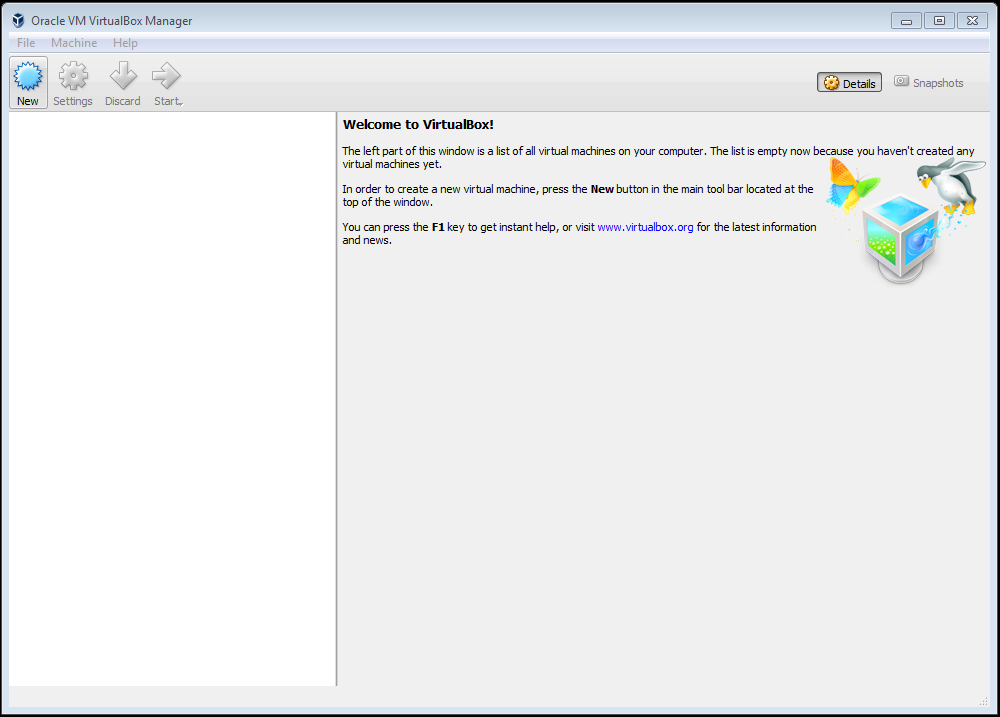
\includegraphics[scale=.6]{Capture1.png}\\
            \begin{itemize}
                
                \item if you have never used this before the list on the left should be empty
                
                \item before you start you should make sure you have an internet connection
                \item before you start you should make sure you have access to a power supply or battery
                
            \end{itemize}
	\newpage
	\item Create New Virtual Machine: \vspace{20mm} \\
      		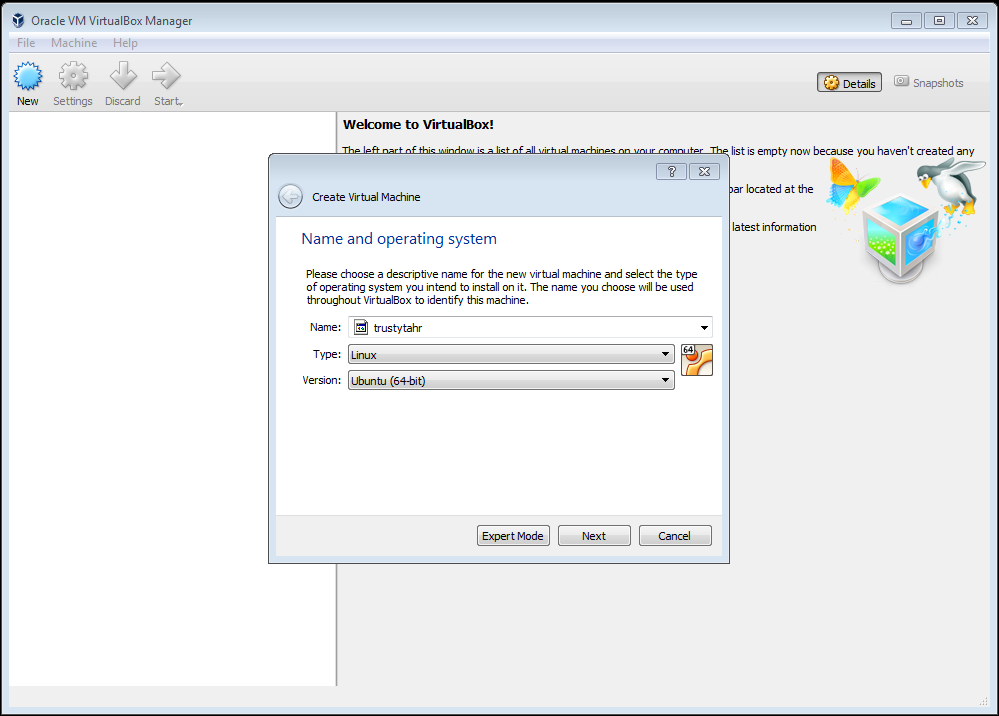
\includegraphics[scale=.6]{Capture2.png}\\
               \begin{itemize}
                
	\item press the {\bf new} button
                \item choose a {\bf computer name} (this is your choice but remember it!)
                \item choose an {\bf operating system} type (Linux)
                \item choose a {\bf version}, this depends on your physical machine This is probably Ubuntu 64-bit but possbily Ubuntu 32-bit) 
                
            \end{itemize}
	\newpage
\item Define Virtual Machine Parameters: \vspace{20mm} \\
      		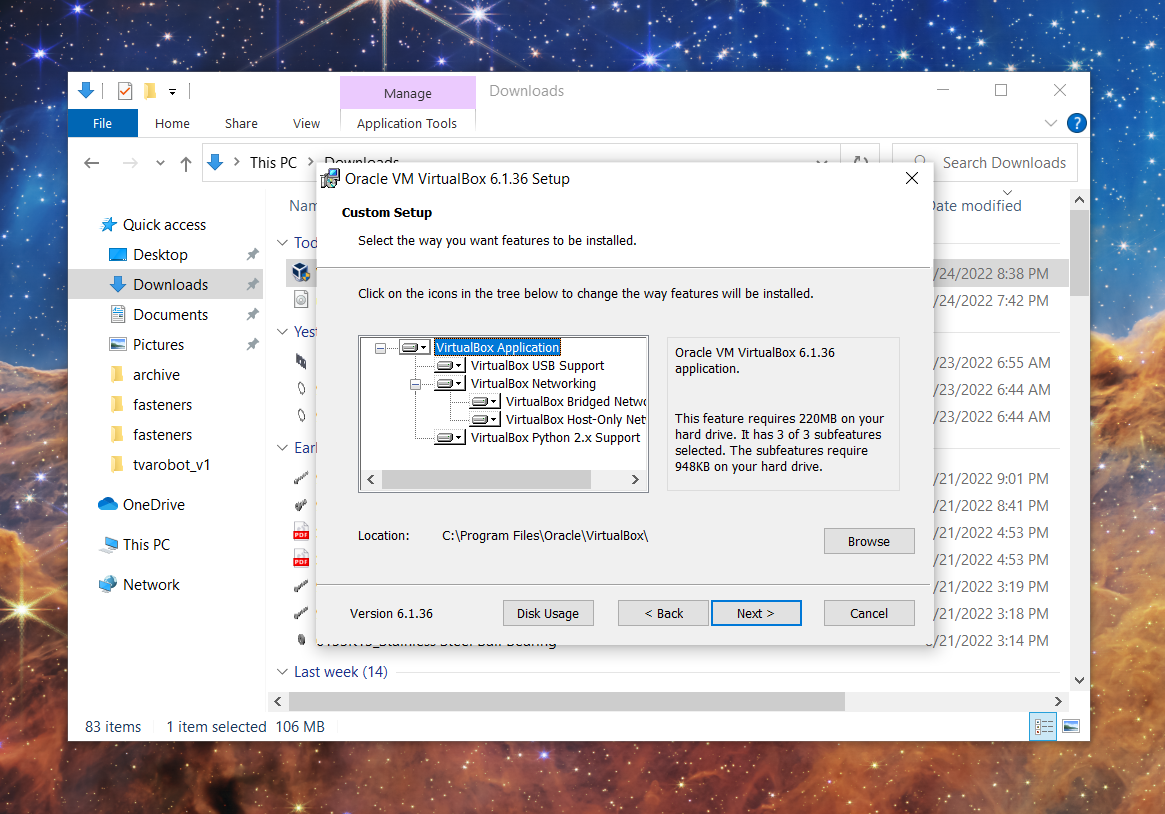
\includegraphics[scale=.6]{Capture3.png}\\
            \begin{itemize}
                
                \item Choose the amount of RAM you want to allocate to the VM
                \item This number is based on your available resources. More is better but it helps to leave some for windows. If your computer has 8GB total I suggest no more than 6GB for for VM.  
                
            \end{itemize}
	\newpage
\item Define Virtual Hard Drive Parameters: \vspace{20mm} \\
      		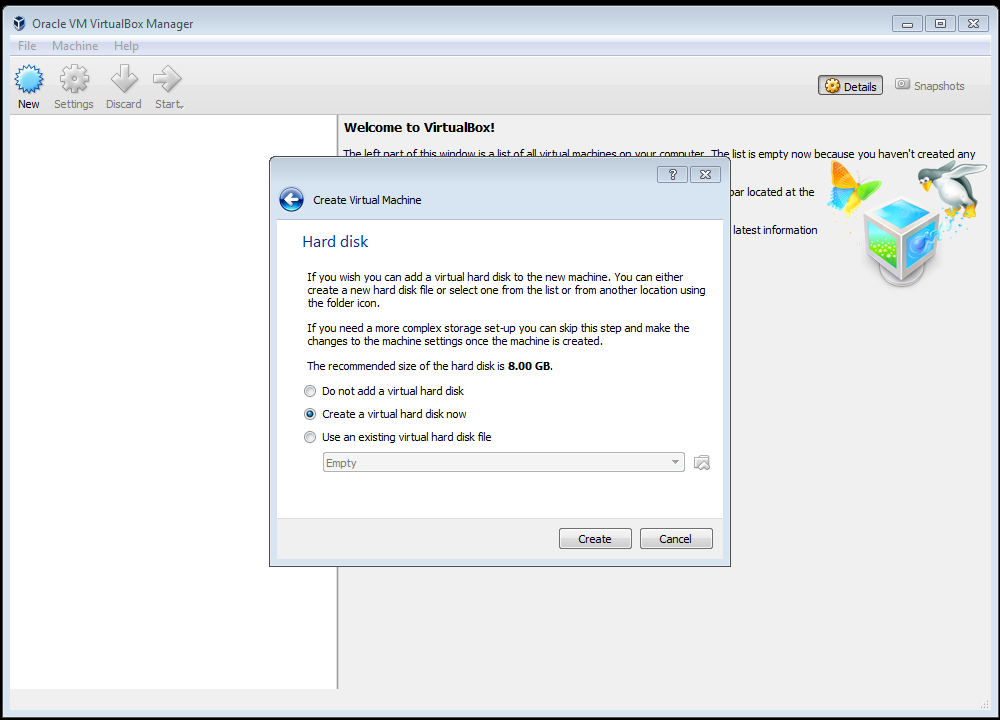
\includegraphics[scale=.6]{Capture4.png}\\
 \begin{itemize}
                
                \item You must have enough space on your hard drive to virutalize linux and install ros. 
                \item {\bf create a virtual hard drive now}
                
            \end{itemize}
	\newpage
\item Virtual Hard Drive Setup: \vspace{20mm} \\
      		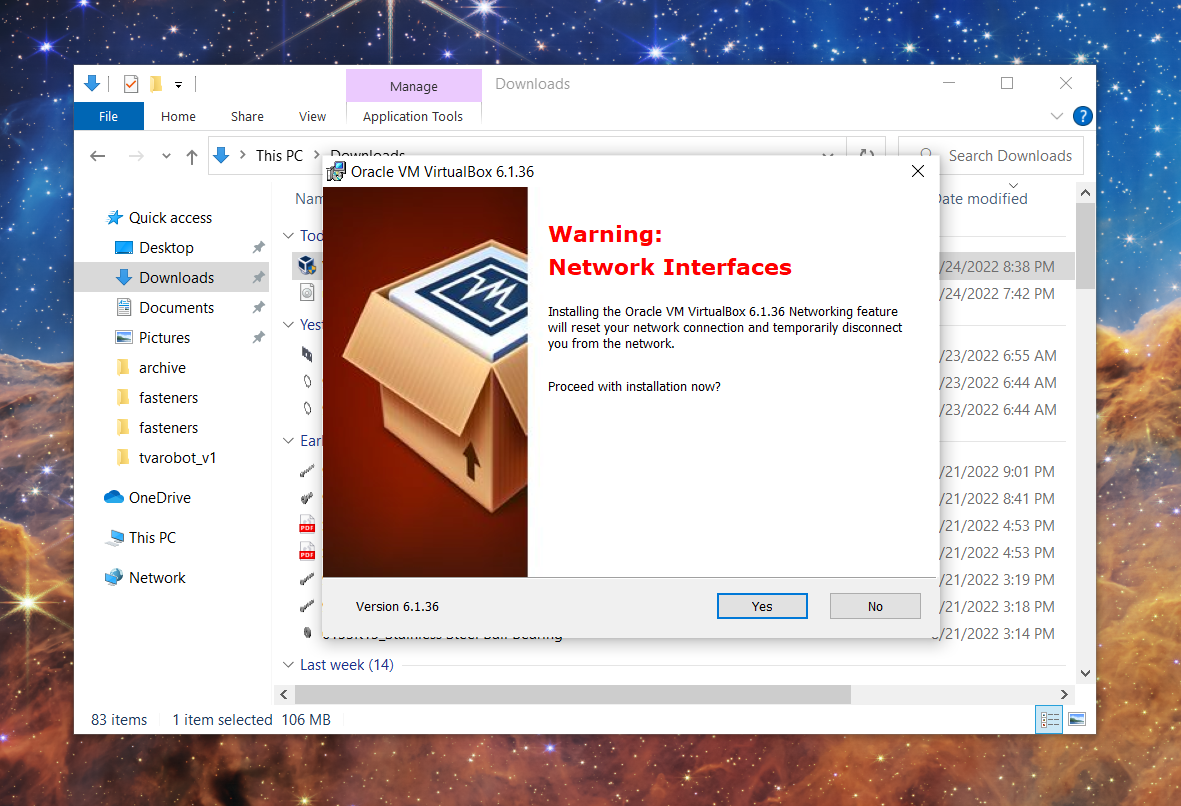
\includegraphics[scale=.6]{Capture5.png}\\
            \begin{itemize}
                
                \item Create a {\bf fixed size} virtual hard drive. 
                              
            \end{itemize}
	\newpage
\item Virtual Hard Drive Setup: \vspace{20mm} \\
        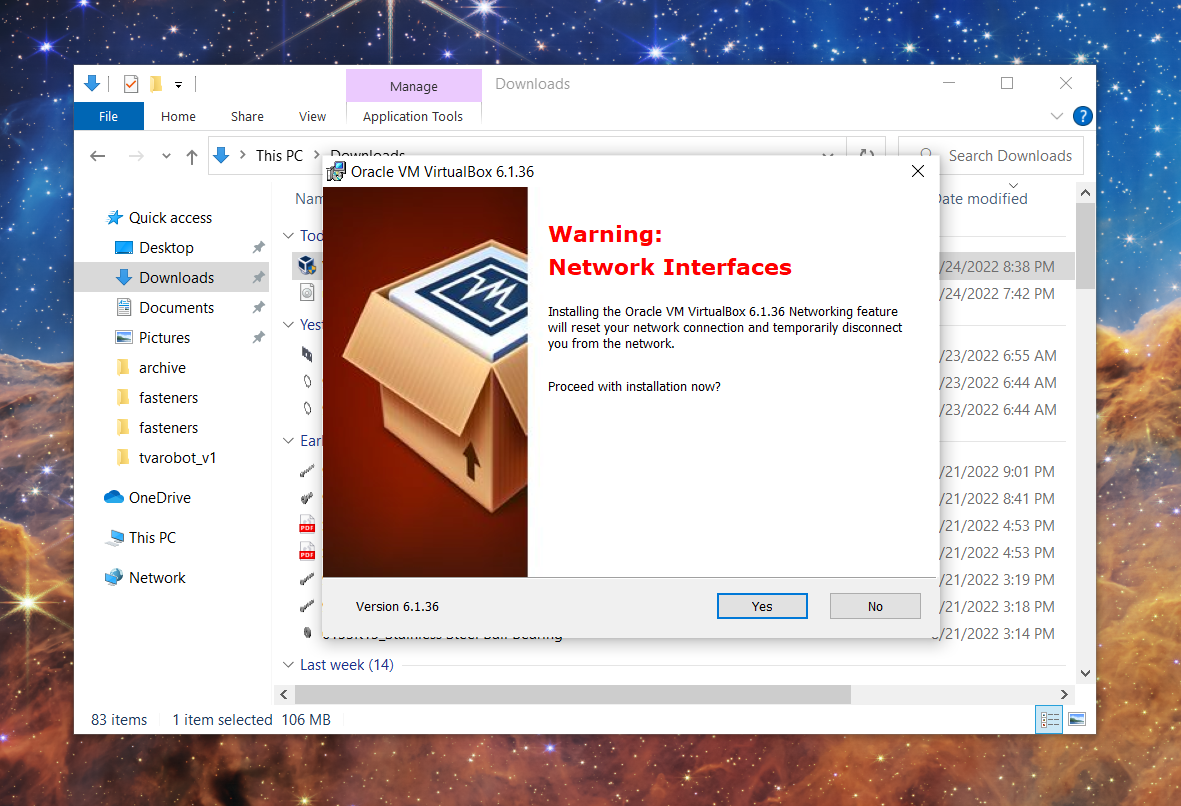
\includegraphics[scale=.6]{Capture5.png}\\
        \begin{itemize}
                        
                \item Choose the virtual hard drive type. 
                \item VDI is recommended.
                           
        \end{itemize}
\newpage
\item Virtual Hard Drive Setup : \vspace{20mm} \\
      		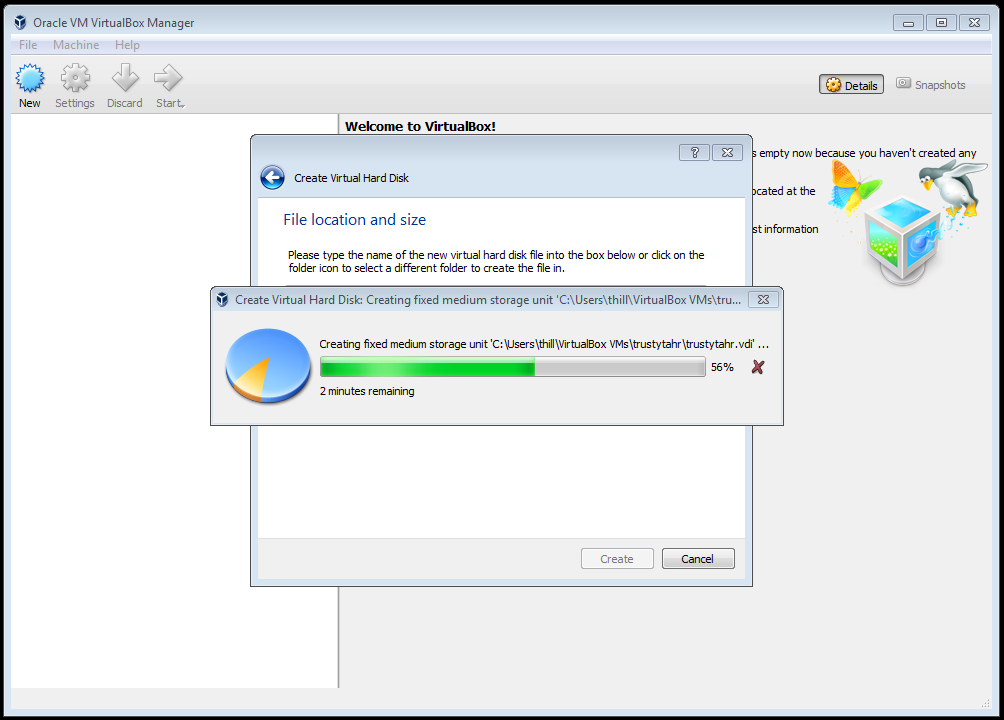
\includegraphics[scale=.6]{Capture6.png}\\
             \begin{itemize}
                    
                \item choose the size of your virtual hard drive       
                \item to virtualize Ubuntu and install ROS it is recommended to make a 16 GB VDI
                \item  you can experiment with 'lighter versions' 
          
                    \begin{itemize}
                            
                        \item lubuntu     
                        \item many more
                        \item I am working on this
                        
                    \end{itemize}
                
            \end{itemize}
	\newpage

\end{enumerate}

		\item[Ubuntu OS Installation and Setup]: \vspace{20mm} \\

\begin{enumerate}
\item Start the VM for the first time: \vspace{20mm} \\
      		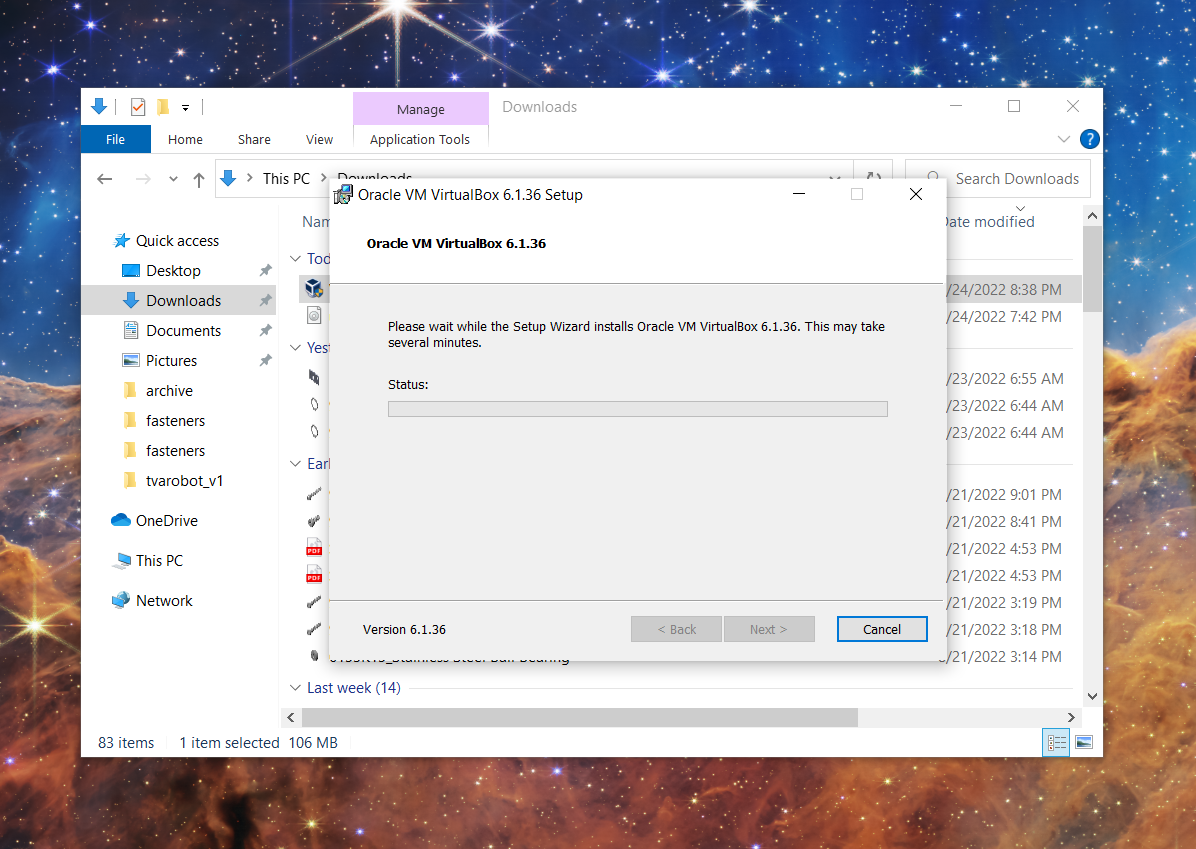
\includegraphics[scale=.6]{Capture7.png}\\
            \begin{itemize}
                    
                 \item select your newly created VM      
                 \item press the green start button
                 \item wait for it...       
            \end{itemize}
	\newpage
\item Start the VM for the first time: \vspace{20mm} \\
      		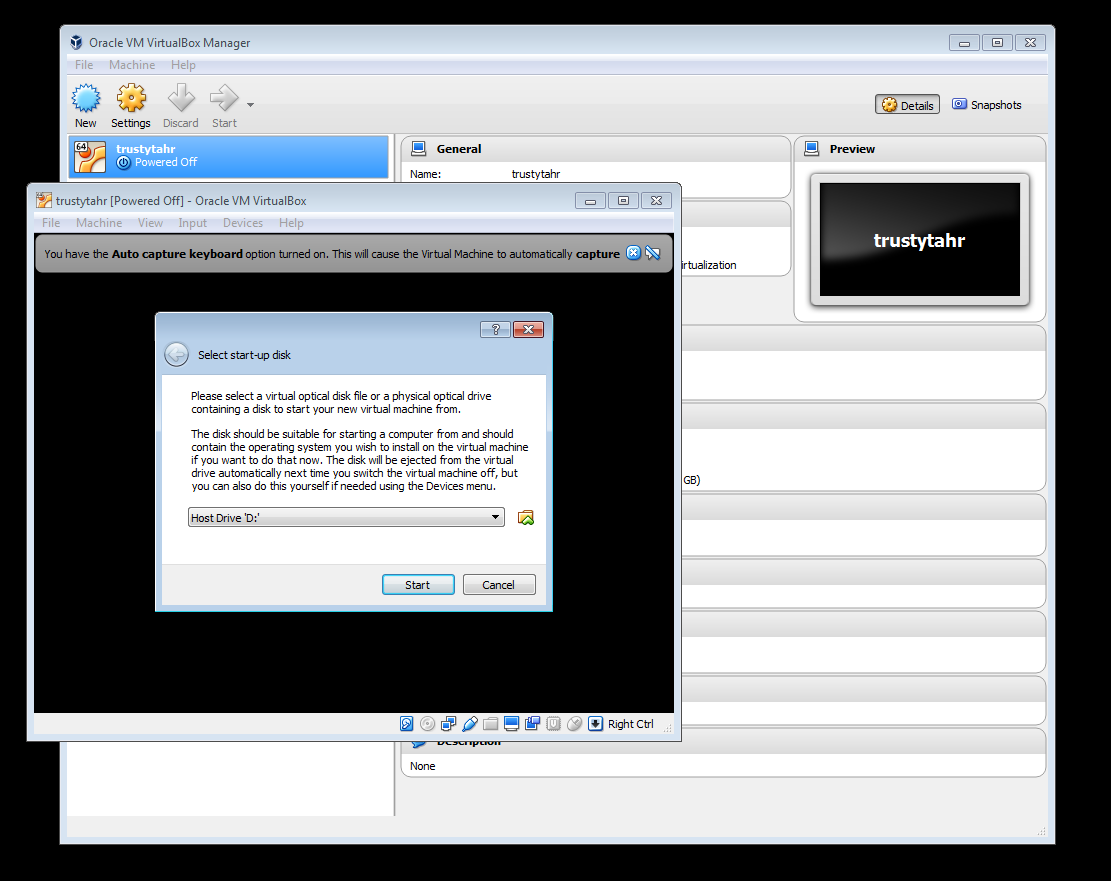
\includegraphics[scale=.6]{Capture8.png}\\
            \begin{itemize}
                    
                 \item choose to select media from a local folder 
                 \item wait for it...
                 
            \end{itemize}
	
\item Start the VM for the first time: \vspace{20mm} \\
      		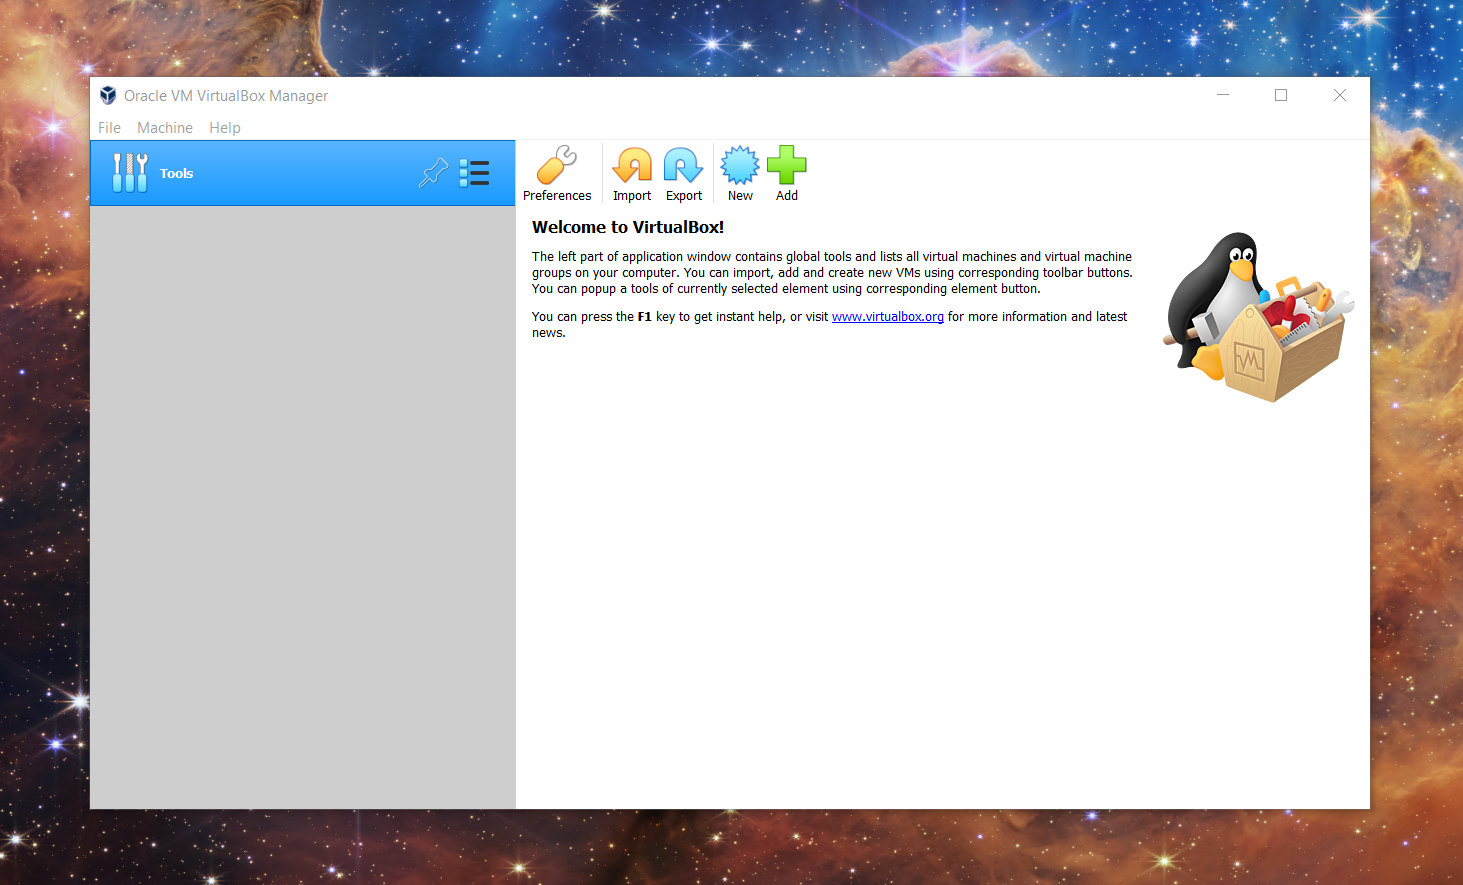
\includegraphics[scale=.6]{Capture9.png} \\
               \begin{itemize}
                    
     
                \item choose the Ubuntu .iso file that you aquired
                \item it is recommended that the media is on the local machine
                \item wait for it...
                
            \end{itemize}


        
	\newpage
\item Ubuntu Installation: \vspace{20mm} \\
      		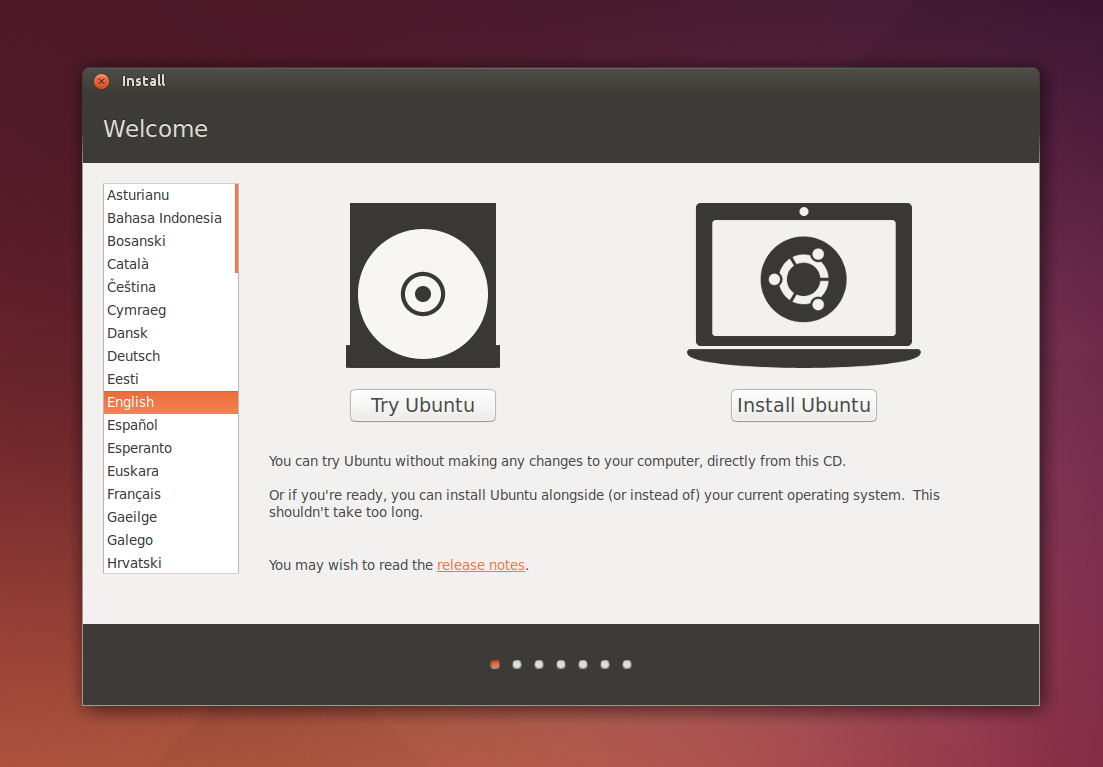
\includegraphics[scale=.6]{Capture10.png}
            \begin{itemize}
                    
                 \item {\bf Install Ubuntu} (harmless if using VirtualBox)
                 \item try is just temporary (single session)
                 \item wait for it...    
            \end{itemize}
	\newpage
\item Ubuntu Installation: \vspace{20mm} \\
      		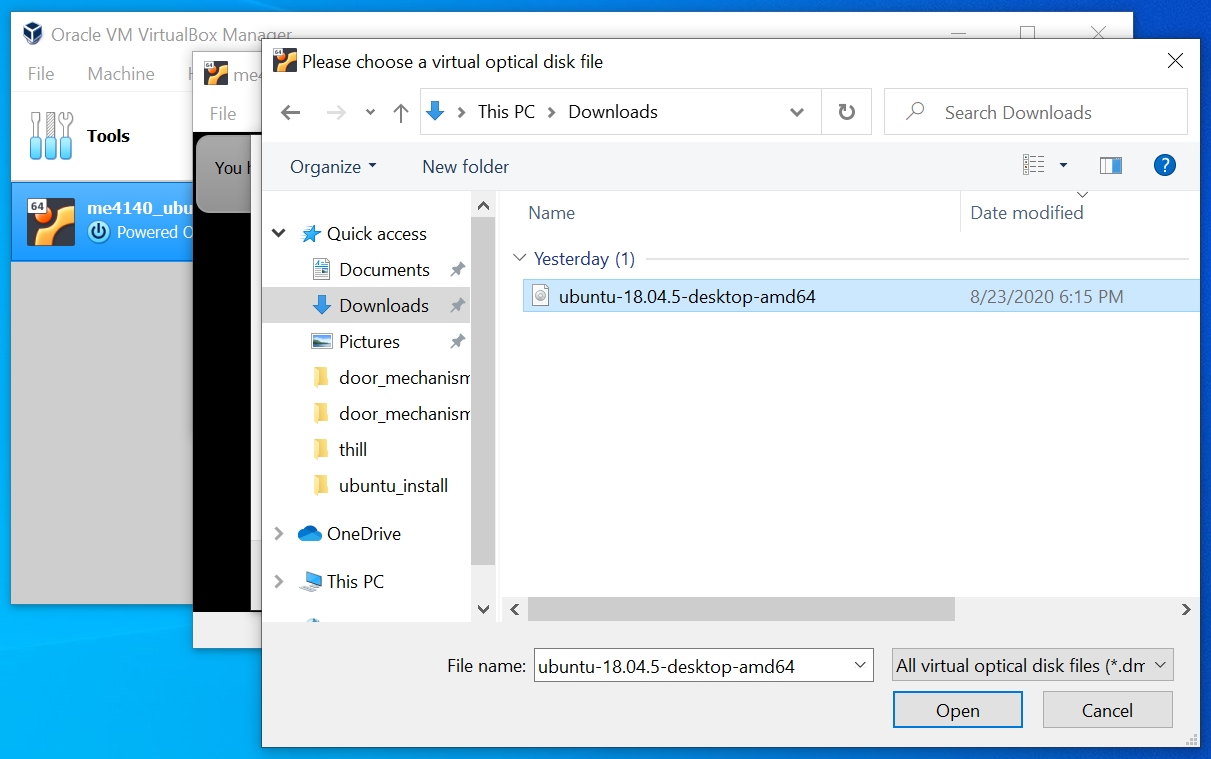
\includegraphics[scale=.6]{Capture11.png} 
            \begin{itemize}
                    \item check that you meet the requirements
                 \item click the two check boxes for proprietary drivers
            \end{itemize}
	\newpage
\item Ubuntu Installation: \vspace{20mm} \\
      		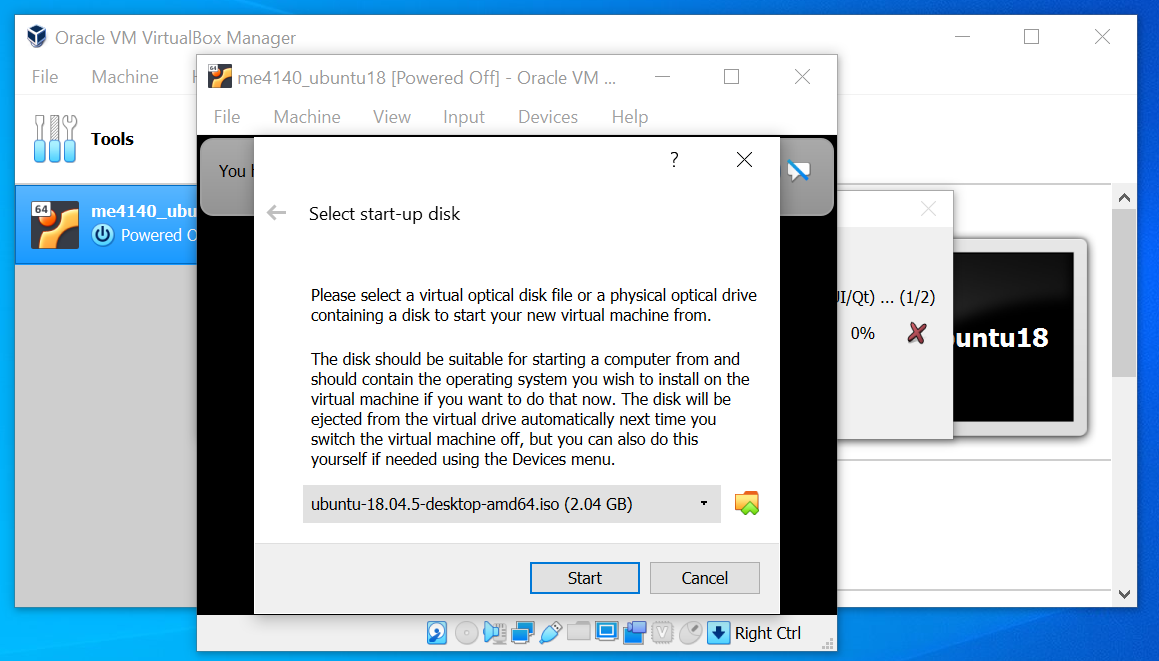
\includegraphics[scale=.6]{Capture12.png}\\
             \begin{itemize}
                    
                 \item {\bf Erase Everything and Install Ubuntu} (harmless if using VirtualBox)
                 \item DANGEROUS AND PERMANENT IF NOT USING VIRTUALBOX
                 \item wait for it...    
            \end{itemize}
	\newpage
\item Wait Wait Wait: \vspace{20mm} \\
      		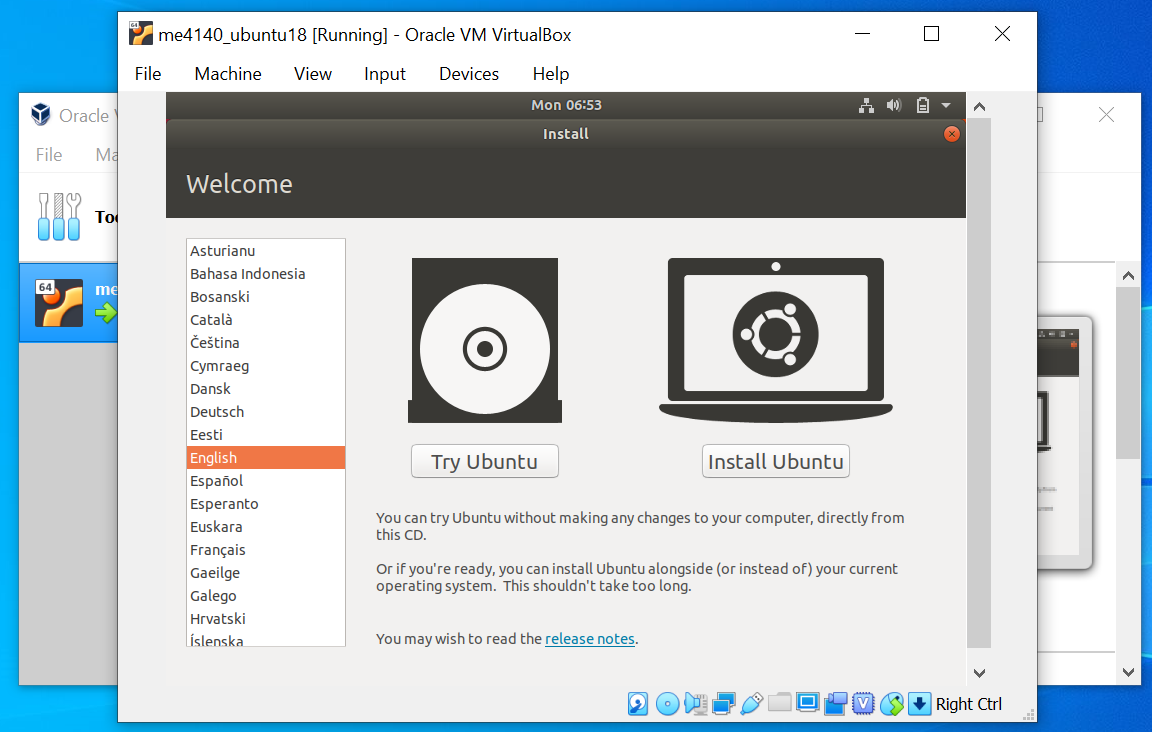
\includegraphics[scale=.6]{Capture13.png}
	\newpage
\item Shut Down The VM: \vspace{20mm} \\
      		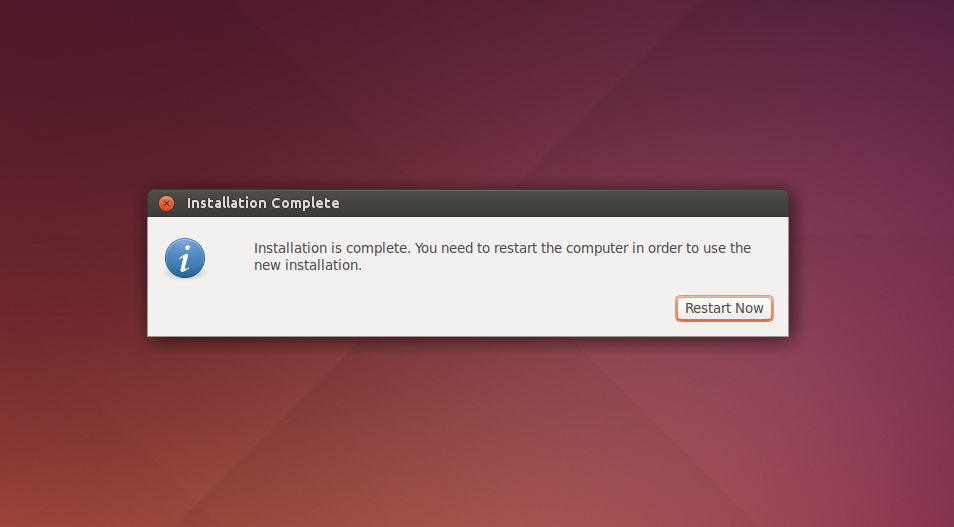
\includegraphics[scale=.6]{Capture14.png}\\
			
	\newpage
\item Shut Down The VM: \vspace{20mm} \\
      		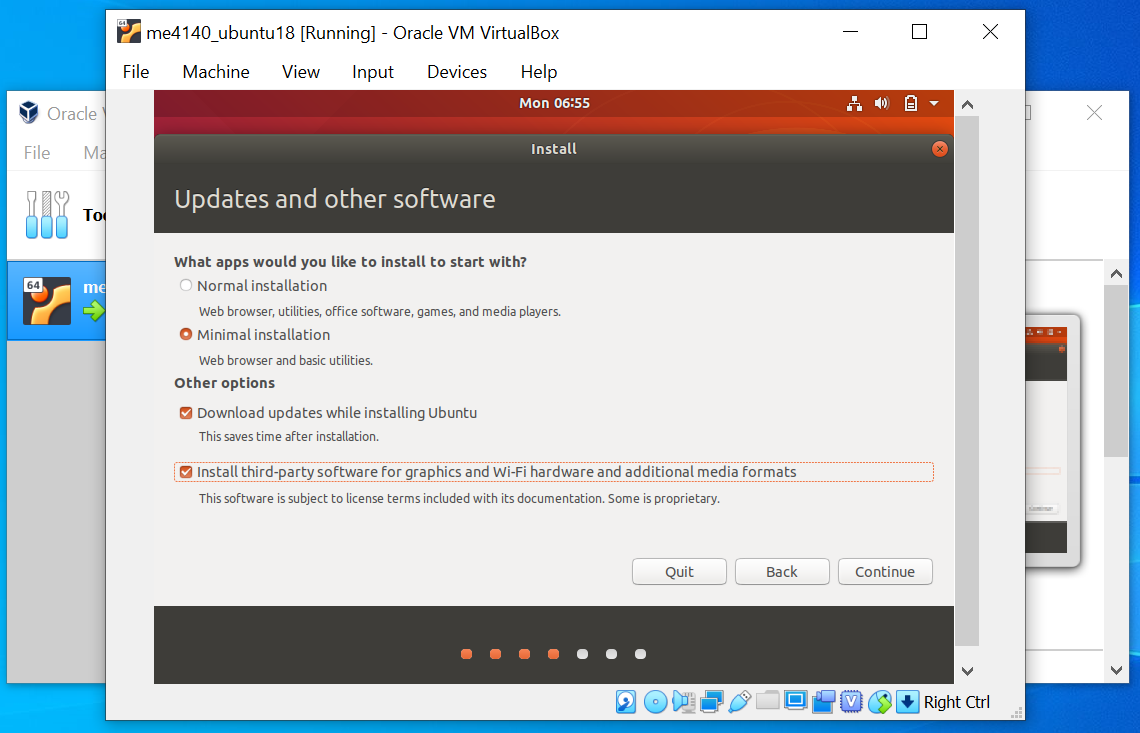
\includegraphics[scale=.6]{Capture15.png}
			\begin{itemize}
                 
				 \item wait for it...
                 \item after waiting a few moments you may have to close the window of the VM
                     
            \end{itemize}
	\newpage
\item Finally!: \vspace{20mm} \\
      		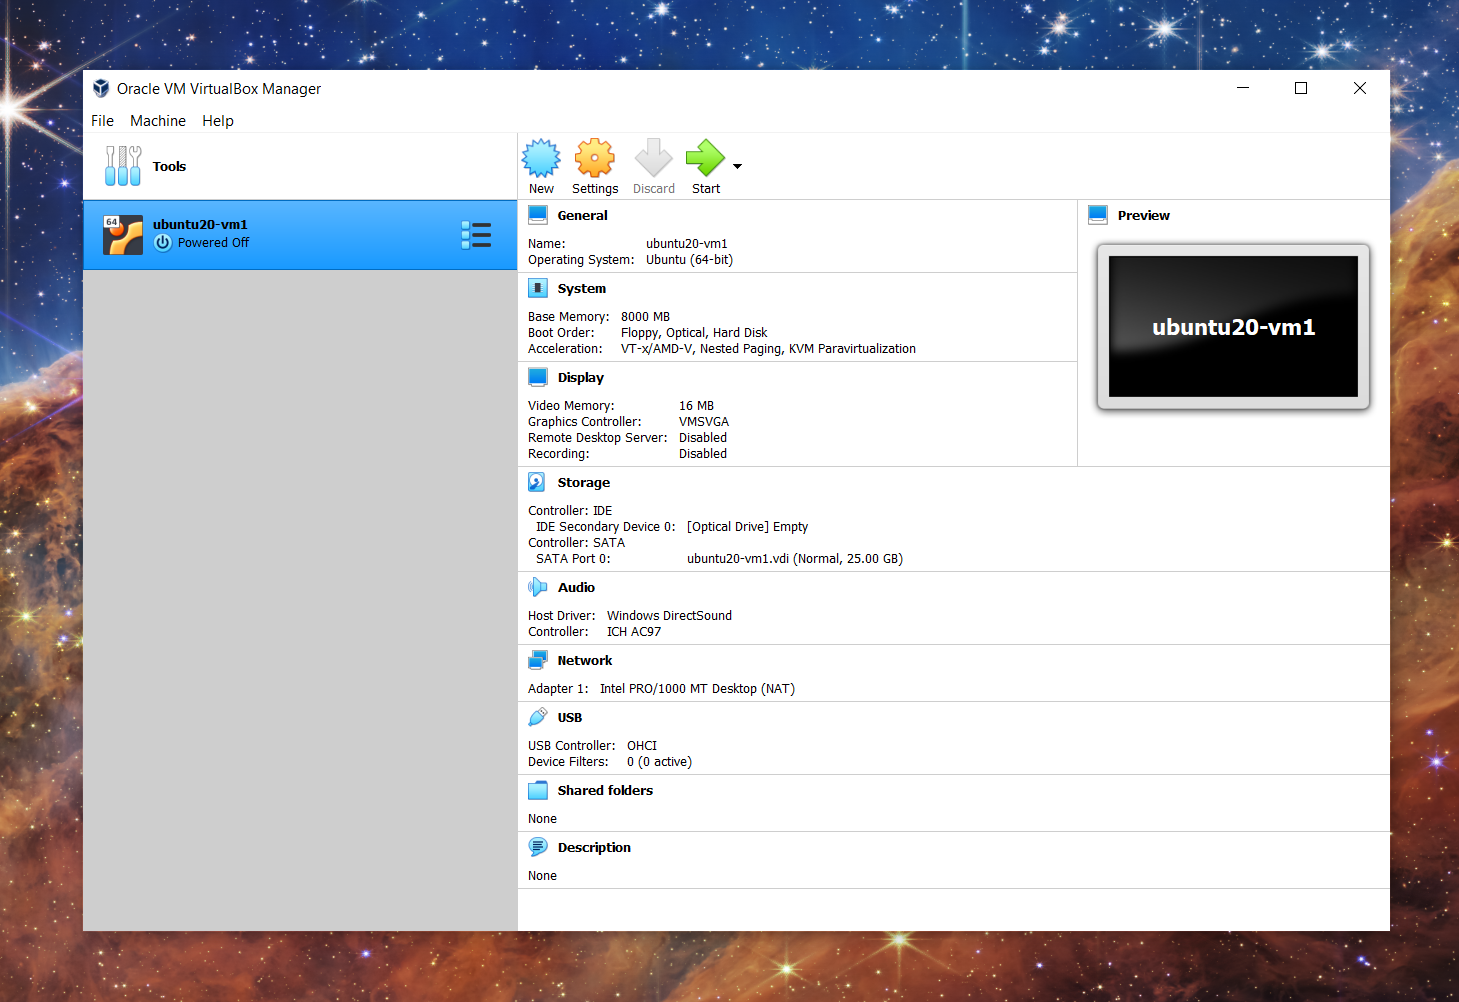
\includegraphics[scale=.6]{Capture16.png}
            \begin{itemize}
        \item POWER OFF the Machine
    \end{itemize} 
	\newpage
\item Now restart the VM!!!:
    \begin{itemize}
        \item the VM you made should be in the left list
        \item select it and click start
		\item the Ubuntu OS should appear	
    \end{itemize}        

\end{enumerate}    
\end{description}
\end{document}

